% Created 2016-01-08 Fri 16:51
\documentclass[bigger]{beamer}
\usepackage[utf8]{inputenc}
\usepackage[T1]{fontenc}
\usepackage{fixltx2e}
\usepackage{graphicx}
\usepackage{grffile}
\usepackage{longtable}
\usepackage{wrapfig}
\usepackage{rotating}
\usepackage[normalem]{ulem}
\usepackage{amsmath}
\usepackage{textcomp}
\usepackage{amssymb}
\usepackage{capt-of}
\usepackage{hyperref}
\usepackage{minted}
\usepackage{inconsolata}
\usepackage{tikz}
\usepgflibrary{shapes.geometric}
\usetikzlibrary{calc}
\usetikzlibrary{positioning}
\usetikzlibrary{plotmarks}
\usepackage{pgfplots}
\mode<beamer>{\usetheme{EPCC}}
\subtitle{preparing for the present}
\institute{EPCC, The University of Edinburgh}
\usetheme{default}
\author{Lawrence Mitchell}
\date{Friday 11th May 2012}
\title{Mixed mode parallelisation of Fluidity}
\hypersetup{
 pdfauthor={Lawrence Mitchell},
 pdftitle={Mixed mode parallelisation of Fluidity},
 pdfkeywords={},
 pdfsubject={},
 pdfcreator={Emacs 24.5.1 (Org mode 8.3.2)}, 
 pdflang={English}}
\AtBeginSection[]{\begin{frame}\tableofcontents[currentsection]\end{frame}}
\begin{document}

\begin{frame}
\maketitle
\end{frame}

\section{Introduction}
\label{sec:orgheadline5}

\begin{frame}[label={sec:orgheadline2}]{Why am I here?}
\begin{itemize}
\item APOS-EU \url{http://www.apos-project.eu/} (EU FP7 project)
\item Performance, and maintainability for multi-/many-core systems
\begin{itemize}
\item Studied through exemplar applications: Fluidity
\end{itemize}
\end{itemize}
\end{frame}

\begin{frame}[label={sec:orgheadline3}]{Big picture}
\begin{itemize}
\item Multicore systems are here to stay
\item \(P \propto V^2 F \propto F^3\)
\item More transistors no longer means faster chips
\item HPC systems are all multi-core (HECToR: 16 (32) cores/node)
\end{itemize}

\begin{center}
\only<2>{
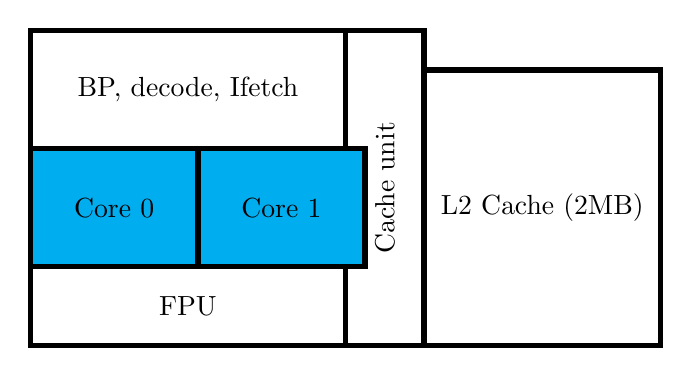
\begin{tikzpicture}
[ele/.style = {rectangle, inner sep = 0, outer sep = 0, line width=2},
core/.style = {draw, fill=cyan}]

\node (module) [ele, minimum
height = 4cm, minimum width = 5 cm, draw] at (0,0) {};

\node (cache) [ele, minimum height
= 3.5cm, minimum width = 3cm, draw, anchor =
south west] at (module.south east) {L2 Cache (2MB)};

\node (FPU) [ele, minimum height = 1cm, minimum width = 4cm, draw,
anchor = south west] at (module.south west) {FPU};

\node (BP) [ele, minimum height = 1.5cm, minimum width = 4cm, draw,
anchor = north west] at (module.north west) {BP, decode, Ifetch};

\node (core0) [ele, core, minimum height = 1.5cm, minimum width =
2.125cm, anchor = south west] at (FPU.north west) {Core 0};

\node (core1) [ele, core, minimum height = 1.5cm, minimum width =
2.125cm, anchor = south west] at (core0.south east) {Core 1};

\draw [line width = 2] (cache.north west) -- +(0, 0.5cm);

\node (cacheunit) [ele, minimum height = 1cm, minimum width = 4cm,
rotate=90, anchor = south west] at (cache.south west) {Cache unit};

\end{tikzpicture}
}
\end{center}
\end{frame}

\begin{frame}[label={sec:orgheadline4}]{What does this mean?}
\begin{itemize}
\item MPI-only works works, but\ldots{}
\item Lose any shared-memory gains (cache-sharing, etc\ldots{})
\item Strong scaling surface-to-volume ratios hurt
\begin{itemize}
\item Easy to have too much halo data
\end{itemize}
\end{itemize}
\end{frame}

\section{Mixed-mode parallelism}
\label{sec:orgheadline9}
\begin{frame}[label={sec:orgheadline6}]{A solution}
\begin{itemize}
\item Mixed-mode/hybrid parallelisation
\item Do shared memory parallelisation on the node
\begin{itemize}
\item or even GPU-like accelerators?
\end{itemize}
\item MPI between nodes
\end{itemize}
\end{frame}

\begin{frame}[label={sec:orgheadline7}]{OpenMP vs. MPI}
\begin{itemize}
\item OpenMP espoused as easier to learn
\item This doesn't translate into easier to program
\item Modelling performance is harder
\item You might need new algorithms
\end{itemize}
\end{frame}

\begin{frame}[label={sec:orgheadline8}]{Algorithmic changes}
\begin{itemize}
\item Distributed memory uses the same algorithm as sequential
\begin{itemize}
\item just (ha!) need data in the right place
\item explicit synchronisation points
\end{itemize}
\item Shared memory has to use different algorithms
\begin{itemize}
\item implicit synchronisation points
\item avoid race conditions
\end{itemize}
\end{itemize}
\end{frame}
\section{Writing threaded code}
\label{sec:orgheadline14}
\begin{frame}[fragile,label={sec:orgheadline10}]{Data races}
 \begin{itemize}
\item Simultaneous writes
\item Read before write/Write before read
\item Generally not this easy to spot!
\end{itemize}
\begin{minted}[frame=none,xleftmargin=1em,xrightmargin=1em,fontsize=\scriptsize]{fortran}
subroutine foo(g)
  g = threadid
end subroutine foo
program main
  integer :: g

  !$OMP parallel
  call foo(g)
  !$OMP end parallel
end program main
\end{minted}

\begin{minted}[frame=none,xleftmargin=1em,xrightmargin=1em,fontsize=\scriptsize]{fortran}
subroutine bar(g)
  g = g + 1
end subroutine bar
program main
  integer :: g
  g = 0
  !$OMP parallel
  call bar(g)
  !$OMP end parallel
end program main
\end{minted}
\end{frame}

\begin{frame}[fragile,label={sec:orgheadline11}]{Getting performance is hard}
 \begin{minted}[frame=none,xleftmargin=1em,xrightmargin=1em,fontsize=\scriptsize]{fortran}
real, dimension(:) :: a, b, c
allocate(a(N), b(N), c(N))
b = 1
c = 2
!$OMP parallel do
do i = 1, N
   a(i) = b(i) + scalar * c(i)
end do
\end{minted}
\begin{itemize}
\item This code is "wrong" on modern systems
\end{itemize}
\end{frame}

\begin{frame}[label={sec:orgheadline12}]{Data layout is important}
\begin{itemize}
\item<1-> HECToR (4 memory nodes)
\item<2-> Serial initialisation
  \begin{itemize}
    \item all data on memory node 0 (22GB/s)
  \end{itemize}
\item<3-> Parallel initialisation
  \begin{itemize}
    \item spread across memory nodes (44GB/s)
  \end{itemize}
\end{itemize}
\begin{center}
\only<1>{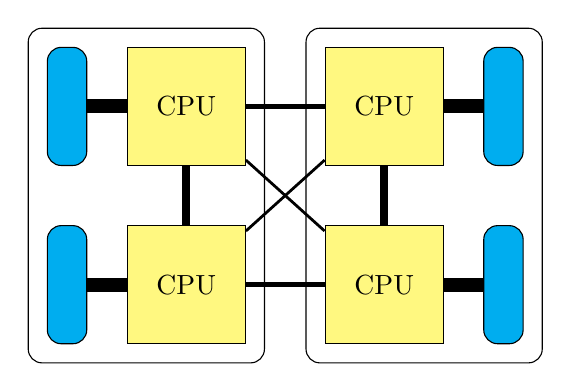
\begin{tikzpicture}[ram/.style={rectangle, inner sep = 0, minimum width=0.5cm, minimum
height = 1.5cm, draw, rounded corners=5pt, fill=cyan},
uma/.style = {rectangle, inner sep = 0, minimum size=1.5cm, draw, fill=yellow!50},
socket/.style = {rectangle, inner sep = 0, rounded corners=5pt, draw}]

\node (RAM1) [ram] at (0,0) {};

\node (RAM2) [ram, below=0.75cm of RAM1] {};

\node (UMA1) [uma, right=0.5cm of RAM1] {CPU};

\node (UMA2) [uma, right=0.5cm of RAM2] {CPU};

\node (UMA3)  [uma, right=1cm of UMA1] {CPU};

\node (UMA4)  [uma, right=1cm of UMA2] {CPU};

\node (RAM3) [ram, right=0.5cm of UMA3] {};

\node (RAM4) [ram, right=0.5cm of UMA4] {};

\node (SOCKET1) [socket, minimum height=4.25cm, minimum
width=3cm, anchor=center] at (intersection of RAM1.north
west--UMA2.south east and RAM2.south west--UMA1.north east) {};
\node (SOCKET2) [socket, minimum height=4.25cm, minimum
width=3cm, anchor=center] at (intersection of UMA3.north
west--RAM4.south east and UMA4.south west--RAM3.north east) {};

\draw [line width=5pt] (RAM1) -- (UMA1);

\draw [line width=5pt] (RAM2) -- (UMA2);
\draw [line width=5pt] (RAM3) -- (UMA3);
\draw [line width=5pt] (RAM4) -- (UMA4);

\draw [line width=3pt] (UMA1) -- (UMA2);
\draw [line width=3pt] (UMA3) -- (UMA4);

\draw [line width=2pt] (UMA1) -- (UMA3);
\draw [line width=2pt] (UMA2) -- (UMA4);

\draw [line width=1pt] (UMA1) -- (UMA4);
\draw [line width=1pt] (UMA2) -- (UMA3);
\end{tikzpicture}
}

\only<2>{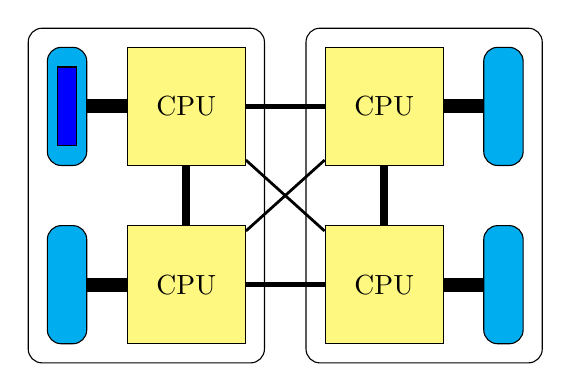
\begin{tikzpicture}[ram/.style={rectangle, inner sep = 0, minimum width=0.5cm, minimum
height = 1.5cm, draw, rounded corners=5pt, fill=cyan},
uma/.style = {rectangle, inner sep = 0, minimum size=1.5cm, draw,
fill=yellow!50},
data/.style = {rectangle, inner sep = 0, minimum width=0.25cm, minimum
height = 1cm, draw, fill=blue},
socket/.style = {rectangle, inner sep = 0, rounded corners=5pt, draw}]

\node (RAM1) [ram] at (0,0) {};

\node (RAM2) [ram, below=0.75cm of RAM1] {};

\node (UMA1) [uma, right=0.5cm of RAM1] {CPU};

\node (UMA2) [uma, right=0.5cm of RAM2] {CPU};

\node (UMA3)  [uma, right=1cm of UMA1] {CPU};

\node (UMA4)  [uma, right=1cm of UMA2] {CPU};

\node (RAM3) [ram, right=0.5cm of UMA3] {};

\node (RAM4) [ram, right=0.5cm of UMA4] {};

\node (data) [data] at (RAM1.center) {};

\node (SOCKET1) [socket, minimum height=4.25cm, minimum
width=3cm, anchor=center] at (intersection of RAM1.north
west--UMA2.south east and RAM2.south west--UMA1.north east) {};
\node (SOCKET2) [socket, minimum height=4.25cm, minimum
width=3cm, anchor=center] at (intersection of UMA3.north
west--RAM4.south east and UMA4.south west--RAM3.north east) {};

\draw [line width=5pt] (RAM1) -- (UMA1);

\draw [line width=5pt] (RAM2) -- (UMA2);
\draw [line width=5pt] (RAM3) -- (UMA3);
\draw [line width=5pt] (RAM4) -- (UMA4);

\draw [line width=3pt] (UMA1) -- (UMA2);
\draw [line width=3pt] (UMA3) -- (UMA4);

\draw [line width=2pt] (UMA1) -- (UMA3);
\draw [line width=2pt] (UMA2) -- (UMA4);

\draw [line width=1pt] (UMA1) -- (UMA4);
\draw [line width=1pt] (UMA2) -- (UMA3);
\end{tikzpicture}
}

\only<3>{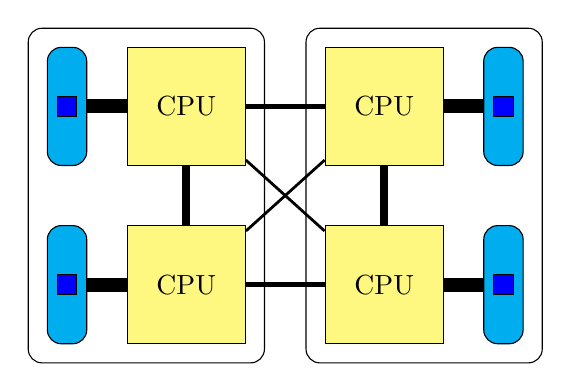
\begin{tikzpicture}[ram/.style={rectangle, inner sep = 0, minimum width=0.5cm, minimum
height = 1.5cm, draw, rounded corners=5pt, fill=cyan},
uma/.style = {rectangle, inner sep = 0, minimum size=1.5cm, draw,
fill=yellow!50},
data/.style = {rectangle, inner sep = 0, minimum width=0.25cm, minimum
height = 0.25cm, draw, fill=blue},
socket/.style = {rectangle, inner sep = 0, rounded corners=5pt, draw}]

\node (RAM1) [ram] at (0,0) {};

\node (RAM2) [ram, below=0.75cm of RAM1] {};

\node (UMA1) [uma, right=0.5cm of RAM1] {CPU};

\node (UMA2) [uma, right=0.5cm of RAM2] {CPU};

\node (UMA3)  [uma, right=1cm of UMA1] {CPU};

\node (UMA4)  [uma, right=1cm of UMA2] {CPU};

\node (RAM3) [ram, right=0.5cm of UMA3] {};

\node (RAM4) [ram, right=0.5cm of UMA4] {};

\foreach \ram in {RAM1, RAM2, RAM3, RAM4}
\node [data] at (\ram.center) {};

\node (SOCKET1) [socket, minimum height=4.25cm, minimum
width=3cm, anchor=center] at (intersection of RAM1.north
west--UMA2.south east and RAM2.south west--UMA1.north east) {};
\node (SOCKET2) [socket, minimum height=4.25cm, minimum
width=3cm, anchor=center] at (intersection of UMA3.north
west--RAM4.south east and UMA4.south west--RAM3.north east) {};

\draw [line width=5pt] (RAM1) -- (UMA1);

\draw [line width=5pt] (RAM2) -- (UMA2);
\draw [line width=5pt] (RAM3) -- (UMA3);
\draw [line width=5pt] (RAM4) -- (UMA4);

\draw [line width=3pt] (UMA1) -- (UMA2);
\draw [line width=3pt] (UMA3) -- (UMA4);

\draw [line width=2pt] (UMA1) -- (UMA3);
\draw [line width=2pt] (UMA2) -- (UMA4);

\draw [line width=1pt] (UMA1) -- (UMA4);
\draw [line width=1pt] (UMA2) -- (UMA3);
\end{tikzpicture}
}
\end{center}
\end{frame}

\begin{frame}[fragile,label={sec:orgheadline13}]{What you should have done}
 \begin{minted}[frame=none,xleftmargin=1em,xrightmargin=1em,fontsize=\scriptsize]{fortran}
real, dimension(:) :: a, b, c
allocate(a(N), b(N), c(N))
!$OMP parallel do
do i = 1, N
   b(i) = 1
   c(i) = 2
end do
!$OMP parallel do
do i = 1, N
   a(i) = b(i) + scalar * c(i)
end do
\end{minted}
\end{frame}

\section{Fluidity}
\label{sec:orgheadline17}
\begin{frame}[label={sec:orgheadline15}]{What takes time in Fluidity?}
\begin{itemize}
\item 40\% matrix assembly
\item 40\% linear solves (sparse linear algebra)
\item 20\% stuff (I/O, bla bla bla)
\end{itemize}
\end{frame}

\begin{frame}[label={sec:orgheadline16}]{What do we want to do?}
\begin{itemize}
\item Shared memory parallelisation of
\begin{itemize}
\item linear solves
\item matrix assembly
\end{itemize}
\item Shared memory can give significant gains for sparse linear algebra
\begin{itemize}
\item e.g. OSKI (UC Berkeley)
\end{itemize}
\item Bigger domains means more coarsening levels in multigrid solvers
\end{itemize}
\end{frame}

\section{Threading the assembly loop\ldots{}}
\label{sec:orgheadline23}
\begin{frame}[label={sec:orgheadline18}]{Matrix assembly}
\begin{itemize}
\item For each element:
\begin{itemize}
\item assemble local element integral (trivially parallel)
\item insert contribution into global matrix (not trivially parallel)
\end{itemize}

\item Each local element integral is independent
\begin{itemize}
\item reads from shared data, but writes to private data
\end{itemize}

\item Insertion into global matrix is not
\begin{itemize}
\item multiple elements may contribute to each dof
\end{itemize}
\end{itemize}

\begin{center}
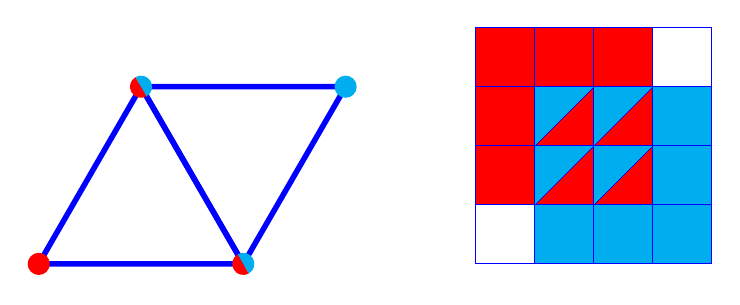
\begin{tikzpicture}
[matrix/.style={rectangle, inner sep = 0, minimum size = 0.75cm, draw =
blue, line width=0, anchor = north east},
element/.style={regular polygon, regular polygon sides=3, draw=blue,
line width=2pt, inner sep=0, outer sep=0, minimum size = 3cm}]

\node (A) [element] at (0,0) {};
\node (B) [element, anchor=corner 1, rotate=180] at
(A.corner 3) {};

\node [circle, fill=red, inner sep = 0, minimum size=8pt] at
(A.corner 2) {};
\node [semicircle, fill=red, line width=0, inner sep = 0, minimum size =4pt, rotate
=120, anchor=south] at
(A.corner 3) {};
\node [semicircle, fill=red, line width=0, inner sep = 0, minimum size =4pt, rotate
=120, anchor=south] at
(A.corner 1) {};


\node [circle, fill=cyan, inner sep=0, minimum size=8pt] at
(B.corner 2) {};
\node [semicircle, fill=cyan, line width=0, inner sep = 0, minimum size =4pt, rotate
=-60, anchor=south] at
(B.corner 3) {};
\node [semicircle, fill=cyan, line width=0, inner sep = 0, minimum size =4pt, rotate
=-60, anchor=south] at
(B.corner 1) {};

\node [matrix]
at (5, 0) {};
\node [matrix, fill=cyan]
at (5.75, 0) {};
\node [matrix, fill=cyan]
at (6.5, 0) {};
\node [matrix, fill=cyan]
at (7.25, 0) {};

\node [matrix, fill=red]
at (5, 0.75) {};
\node (M1) [matrix]
at (5.75, 0.75) {};
\node (M2) [matrix]
at (6.5, 0.75) {};
\node [matrix, fill=cyan]
at (7.25, 0.75) {};

\node [matrix, fill=red]
at (5, 1.5) {};
\node (M3) [matrix]
at (5.75, 1.5) {};
\node (M4) [matrix]
at (6.5, 1.5) {};
\node [matrix, fill=cyan]
at (7.25, 1.5) {};

\foreach \thing in {M1, M2, M3, M4}
{
\draw [fill=cyan, line width=0, draw=blue] (\thing.south west) --
(\thing.north east) -- (\thing.north west) -- cycle;

\draw [fill=red, line width=0, draw=blue] (\thing.south west) --
(\thing.north east) -- (\thing.south east) -- cycle;
}
\node [matrix, fill=red]
at (5, 2.25) {};
\node [matrix, fill=red]
at (5.75, 2.25) {};
\node [matrix, fill=red]
at (6.5, 2.25) {};
\node [matrix]
at (7.25, 2.25) {};

\end{tikzpicture}
\end{center}
\end{frame}

\begin{frame}[fragile,label={sec:orgheadline19}]{How to avoid the race condition?}
 \begin{itemize}
\item Make global matrix insertion "critical"
\begin{itemize}
\item only one thread can update at a time
\end{itemize}
\end{itemize}
\begin{minted}[frame=none,xleftmargin=1em,xrightmargin=1em,fontsize=\scriptsize]{fortran}
!$OMP parallel do
do ele = 1, nele
   localtensor = assemble(ele)
   !$OMP critical
   call addto(localtensor, big_matrix)
end do
\end{minted}

\begin{itemize}
\item No!  This will give awful performance
\end{itemize}
\end{frame}

\begin{frame}[fragile,label={sec:orgheadline20}]{Solutions II}
 \begin{itemize}
\item Make insertion of an entry "atomic"
\end{itemize}
\begin{minted}[frame=none,xleftmargin=1em,xrightmargin=1em,fontsize=\scriptsize]{fortran}
subroutine addto(ltensor, m)
  ...
  !$OMP atomic
  m%data(i,j) = m%data(i,j) + ltensor
  ...
end subroutine addto
\end{minted}

\begin{itemize}
\item still bad, most OMP implementations lock \texttt{matrix\%data}, not
\texttt{matrix\%data(i,j)}
\end{itemize}
\end{frame}

\begin{frame}[label={sec:orgheadline21}]{Solutions III}
\begin{itemize}
\item Write your code in a race-free fashion
\begin{itemize}
\item ensure that no two threads will ever update the same dof
simultaneously
\end{itemize}
\item Mesh colouring
\begin{itemize}
\item Colour elements such that elements that share dofs have different
colours
\end{itemize}
\end{itemize}

\begin{center}
\only<1>{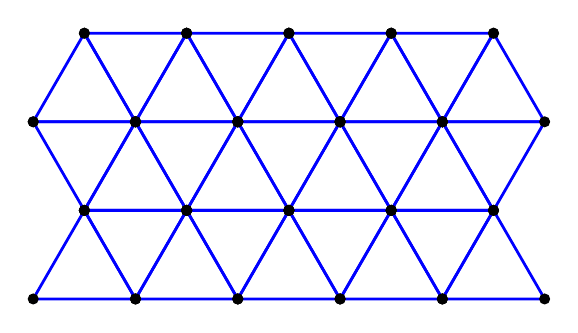
\begin{tikzpicture}[element/.style = {regular
polygon, regular polygon sides=3, draw=blue, line width=1pt, 
inner sep = 0, outer sep = 0, minimum size=1.5cm},
dof/.style = {circle, inner sep=0, fill=black, minimum size = 4pt}]

\node (A) [element] at
(0,0) {};
\node (B) [element, anchor=corner 1, rotate=180] at
(A.corner 3) {};
\node (C) [element, anchor=corner 2] at (A.corner 3) {};
\node (D) [element, anchor=corner 1, rotate=180] at
(C.corner 3) {};
\node (E) [element, anchor=corner 2] at (C.corner 3) {};

\node (F) [element, anchor=corner 1, rotate=180] at
(E.corner 3) {};
\node (G) [element, anchor=corner 2] at (E.corner 3) {};

\node (H) [element, anchor=corner 1, rotate=180] at
(G.corner 3) {};
\node (I) [element, anchor=corner 2] at (G.corner 3) {};

\node (A1) [element, rotate=180, anchor=corner 3] at
(A.corner 2) {};
\node (B1) [element, anchor=corner 2] at
(A1.corner 1) {};

\node (C1) [element, rotate=180, anchor=corner 3] at
(C.corner 2) {};
\node (D1) [element, anchor=corner 2] at
(C1.corner 1) {};

\node (E1) [element, rotate=180, anchor=corner 3] at
(E.corner 2) {};
\node (F1) [element, anchor=corner 2] at
(E1.corner 1) {};

\node (G1) [element, rotate=180, anchor=corner 3] at
(G.corner 2) {};
\node (H1) [element, anchor=corner 2] at
(G1.corner 1) {};
\node (I1) [element, rotate=180, anchor=corner 3] at
(I.corner 2) {};

\node (A2) [element, anchor=corner 1] at
(A1.corner 1) {};
\node (B2) [element, anchor=corner 1, rotate=180] at
(A2.corner 3) {};
\node (C2) [element, anchor=corner 2] at (A2.corner 3) {};
\node (D2) [element, anchor=corner 1, rotate=180] at
(C2.corner 3) {};
\node (E2) [element, anchor=corner 2] at (C2.corner 3) {};

\node (F2) [element, anchor=corner 1, rotate=180] at
(E2.corner 3) {};
\node (G2) [element, anchor=corner 2] at (E2.corner 3) {};

\node (H2) [element, anchor=corner 1, rotate=180] at
(G2.corner 3) {};
\node (I2) [element, anchor=corner 2] at (G2.corner 3) {};

\foreach \ele in {A, B, C, D, E, F, G, H, I,
                  A1, B1, C1, D1, E1, F1, G1, H1,
                  A2, B2, C2, D2, E2, F2, G2, H2, I2}
\foreach \val in {corner 1, corner 2, corner 3}
\node [dof] at (\ele.\val) {};
\end{tikzpicture}
}

\only<2>{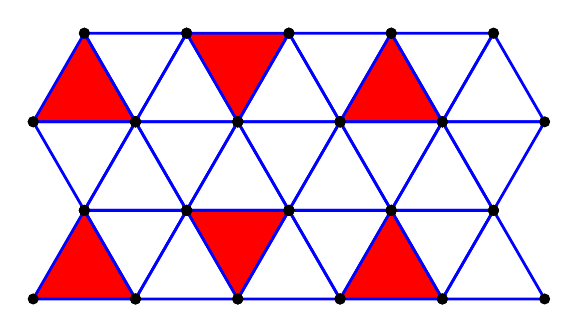
\begin{tikzpicture}[element/.style = {regular
polygon, regular polygon sides=3, draw=blue, line width=1pt, 
inner sep = 0, outer sep = 0, minimum size=1.5cm},
dof/.style = {circle, inner sep=0, fill=black, minimum size = 4pt}]

\node (A) [element, fill=red] at
(0,0) {};
\node (B) [element, anchor=corner 1, rotate=180] at
(A.corner 3) {};
\node (C) [element, anchor=corner 2] at (A.corner 3) {};
\node (D) [element, anchor=corner 1, rotate=180, fill=red] at
(C.corner 3) {};
\node (E) [element, anchor=corner 2] at (C.corner 3) {};

\node (F) [element, anchor=corner 1, rotate=180] at
(E.corner 3) {};
\node (G) [element, anchor=corner 2, fill=red] at (E.corner 3) {};

\node (H) [element, anchor=corner 1, rotate=180] at
(G.corner 3) {};
\node (I) [element, anchor=corner 2] at (G.corner 3) {};

\node (A1) [element, rotate=180, anchor=corner 3] at
(A.corner 2) {};
\node (B1) [element, anchor=corner 2] at
(A1.corner 1) {};

\node (C1) [element, rotate=180, anchor=corner 3] at
(C.corner 2) {};
\node (D1) [element, anchor=corner 2] at
(C1.corner 1) {};

\node (E1) [element, rotate=180, anchor=corner 3] at
(E.corner 2) {};
\node (F1) [element, anchor=corner 2] at
(E1.corner 1) {};

\node (G1) [element, rotate=180, anchor=corner 3] at
(G.corner 2) {};
\node (H1) [element, anchor=corner 2] at
(G1.corner 1) {};
\node (I1) [element, rotate=180, anchor=corner 3] at
(I.corner 2) {};

\node (A2) [element, anchor=corner 1, fill=red] at
(A1.corner 1) {};
\node (B2) [element, anchor=corner 1, rotate=180] at
(A2.corner 3) {};
\node (C2) [element, anchor=corner 2] at (A2.corner 3) {};
\node (D2) [element, anchor=corner 1, rotate=180, fill=red] at
(C2.corner 3) {};
\node (E2) [element, anchor=corner 2] at (C2.corner 3) {};

\node (F2) [element, anchor=corner 1, rotate=180] at
(E2.corner 3) {};
\node (G2) [element, anchor=corner 2, fill=red] at (E2.corner 3) {};

\node (H2) [element, anchor=corner 1, rotate=180] at
(G2.corner 3) {};
\node (I2) [element, anchor=corner 2] at (G2.corner 3) {};

\foreach \ele in {A, B, C, D, E, F, G, H, I,
                  A1, B1, C1, D1, E1, F1, G1, H1,
                  A2, B2, C2, D2, E2, F2, G2, H2, I2}
\foreach \val in {corner 1, corner 2, corner 3}
\node [dof] at (\ele.\val) {};
\end{tikzpicture}
}

\only<3>{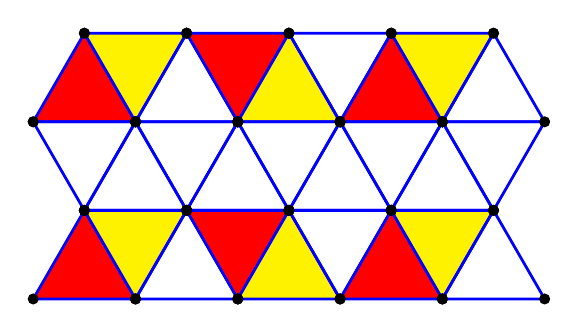
\begin{tikzpicture}[element/.style = {regular
polygon, regular polygon sides=3, draw=blue, line width=1pt, 
inner sep = 0, outer sep = 0, minimum size = 1.5cm},
dof/.style = {circle, inner sep=0, fill=black, minimum size = 4pt}]

\node (A) [element, fill=red] at
(0,0) {};
\node (B) [element, anchor=corner 1, rotate=180, fill=yellow] at
(A.corner 3) {};
\node (C) [element, anchor=corner 2] at (A.corner 3) {};
\node (D) [element, anchor=corner 1, rotate=180, fill=red] at
(C.corner 3) {};
\node (E) [element, anchor=corner 2, fill=yellow] at (C.corner 3) {};

\node (F) [element, anchor=corner 1, rotate=180] at
(E.corner 3) {};
\node (G) [element, anchor=corner 2, fill=red] at (E.corner 3) {};

\node (H) [element, anchor=corner 1, rotate=180, fill=yellow] at
(G.corner 3) {};
\node (I) [element, anchor=corner 2] at (G.corner 3) {};

\node (A1) [element, rotate=180, anchor=corner 3] at
(A.corner 2) {};
\node (B1) [element, anchor=corner 2] at
(A1.corner 1) {};

\node (C1) [element, rotate=180, anchor=corner 3] at
(C.corner 2) {};
\node (D1) [element, anchor=corner 2] at
(C1.corner 1) {};

\node (E1) [element, rotate=180, anchor=corner 3] at
(E.corner 2) {};
\node (F1) [element, anchor=corner 2] at
(E1.corner 1) {};

\node (G1) [element, rotate=180, anchor=corner 3] at
(G.corner 2) {};
\node (H1) [element, anchor=corner 2] at
(G1.corner 1) {};
\node (I1) [element, rotate=180, anchor=corner 3] at
(I.corner 2) {};

\node (A2) [element, anchor=corner 1, fill=red] at
(A1.corner 1) {};
\node (B2) [element, anchor=corner 1, rotate=180, fill=yellow] at
(A2.corner 3) {};
\node (C2) [element, anchor=corner 2] at (A2.corner 3) {};
\node (D2) [element, anchor=corner 1, rotate=180, fill=red] at
(C2.corner 3) {};
\node (E2) [element, anchor=corner 2, fill=yellow] at (C2.corner 3) {};

\node (F2) [element, anchor=corner 1, rotate=180] at
(E2.corner 3) {};
\node (G2) [element, anchor=corner 2, fill=red] at (E2.corner 3) {};

\node (H2) [element, anchor=corner 1, rotate=180, fill=yellow] at
(G2.corner 3) {};
\node (I2) [element, anchor=corner 2] at (G2.corner 3) {};

\foreach \ele in {A, B, C, D, E, F, G, H, I,
                  A1, B1, C1, D1, E1, F1, G1, H1,
                  A2, B2, C2, D2, E2, F2, G2, H2, I2}
\foreach \val in {corner 1, corner 2, corner 3}
\node [dof] at (\ele.\val) {};
\end{tikzpicture}
}

\only<4>{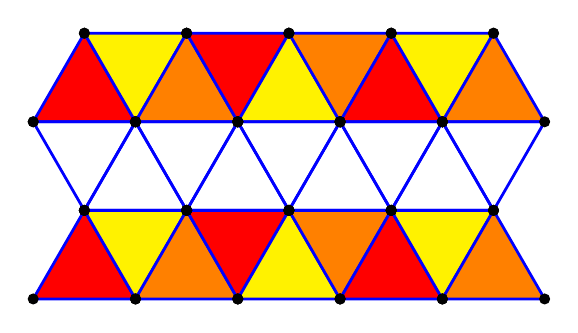
\begin{tikzpicture}[element/.style = {regular
polygon, regular polygon sides=3, draw=blue, line width=1pt, 
inner sep = 0, outer sep = 0, minimum size = 1.5cm},
dof/.style = {circle, inner sep=0, fill=black, minimum size = 4pt}]

\node (A) [element, fill=red] at
(0,0) {};
\node (B) [element, anchor=corner 1, rotate=180, fill=yellow] at
(A.corner 3) {};
\node (C) [element, anchor=corner 2,fill=orange] at (A.corner 3) {};
\node (D) [element, anchor=corner 1, rotate=180, fill=red] at
(C.corner 3) {};
\node (E) [element, anchor=corner 2, fill=yellow] at (C.corner 3) {};

\node (F) [element, anchor=corner 1, rotate=180, fill=orange] at
(E.corner 3) {};
\node (G) [element, anchor=corner 2, fill=red] at (E.corner 3) {};

\node (H) [element, anchor=corner 1, rotate=180, fill=yellow] at
(G.corner 3) {};
\node (I) [element, anchor=corner 2, fill=orange] at (G.corner 3) {};

\node (A1) [element, rotate=180, anchor=corner 3] at
(A.corner 2) {};
\node (B1) [element, anchor=corner 2] at
(A1.corner 1) {};

\node (C1) [element, rotate=180, anchor=corner 3] at
(C.corner 2) {};
\node (D1) [element, anchor=corner 2] at
(C1.corner 1) {};

\node (E1) [element, rotate=180, anchor=corner 3] at
(E.corner 2) {};
\node (F1) [element, anchor=corner 2] at
(E1.corner 1) {};

\node (G1) [element, rotate=180, anchor=corner 3] at
(G.corner 2) {};
\node (H1) [element, anchor=corner 2] at
(G1.corner 1) {};
\node (I1) [element, rotate=180, anchor=corner 3] at
(I.corner 2) {};

\node (A2) [element, anchor=corner 1, fill=red] at
(A1.corner 1) {};
\node (B2) [element, anchor=corner 1, rotate=180, fill=yellow] at
(A2.corner 3) {};
\node (C2) [element, anchor=corner 2, fill=orange] at (A2.corner 3) {};
\node (D2) [element, anchor=corner 1, rotate=180, fill=red] at
(C2.corner 3) {};
\node (E2) [element, anchor=corner 2, fill=yellow] at (C2.corner 3) {};

\node (F2) [element, anchor=corner 1, rotate=180, fill=orange] at
(E2.corner 3) {};
\node (G2) [element, anchor=corner 2, fill=red] at (E2.corner 3) {};

\node (H2) [element, anchor=corner 1, rotate=180, fill=yellow] at
(G2.corner 3) {};
\node (I2) [element, anchor=corner 2, fill=orange] at (G2.corner 3) {};

\foreach \ele in {A, B, C, D, E, F, G, H, I,
                  A1, B1, C1, D1, E1, F1, G1, H1,
                  A2, B2, C2, D2, E2, F2, G2, H2, I2}
\foreach \val in {corner 1, corner 2, corner 3}
\node [dof] at (\ele.\val) {};
\end{tikzpicture}
}

\only<5>{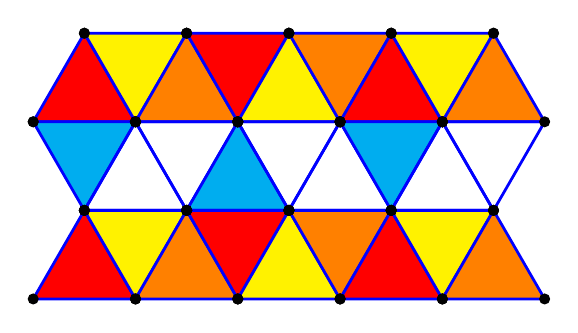
\begin{tikzpicture}[element/.style = {regular
polygon, regular polygon sides=3, draw=blue, line width=1pt, 
inner sep = 0, outer sep = 0, minimum size = 1.5cm},
dof/.style = {circle, inner sep=0, fill=black, minimum size = 4pt}]

\node (A) [element, fill=red] at
(0,0) {};
\node (B) [element, anchor=corner 1, rotate=180, fill=yellow] at
(A.corner 3) {};
\node (C) [element, anchor=corner 2,fill=orange] at (A.corner 3) {};
\node (D) [element, anchor=corner 1, rotate=180, fill=red] at
(C.corner 3) {};
\node (E) [element, anchor=corner 2, fill=yellow] at (C.corner 3) {};

\node (F) [element, anchor=corner 1, rotate=180, fill=orange] at
(E.corner 3) {};
\node (G) [element, anchor=corner 2, fill=red] at (E.corner 3) {};

\node (H) [element, anchor=corner 1, rotate=180, fill=yellow] at
(G.corner 3) {};
\node (I) [element, anchor=corner 2, fill=orange] at (G.corner 3) {};

\node (A1) [element, rotate=180, anchor=corner 3, fill=cyan] at
(A.corner 2) {};
\node (B1) [element, anchor=corner 2] at
(A1.corner 1) {};

\node (C1) [element, rotate=180, anchor=corner 3] at
(C.corner 2) {};
\node (D1) [element, anchor=corner 2, fill=cyan] at
(C1.corner 1) {};

\node (E1) [element, rotate=180, anchor=corner 3] at
(E.corner 2) {};
\node (F1) [element, anchor=corner 2] at
(E1.corner 1) {};

\node (G1) [element, rotate=180, anchor=corner 3, fill=cyan] at
(G.corner 2) {};
\node (H1) [element, anchor=corner 2] at
(G1.corner 1) {};
\node (I1) [element, rotate=180, anchor=corner 3] at
(I.corner 2) {};

\node (A2) [element, anchor=corner 1, fill=red] at
(A1.corner 1) {};
\node (B2) [element, anchor=corner 1, rotate=180, fill=yellow] at
(A2.corner 3) {};
\node (C2) [element, anchor=corner 2, fill=orange] at (A2.corner 3) {};
\node (D2) [element, anchor=corner 1, rotate=180, fill=red] at
(C2.corner 3) {};
\node (E2) [element, anchor=corner 2, fill=yellow] at (C2.corner 3) {};

\node (F2) [element, anchor=corner 1, rotate=180, fill=orange] at
(E2.corner 3) {};
\node (G2) [element, anchor=corner 2, fill=red] at (E2.corner 3) {};

\node (H2) [element, anchor=corner 1, rotate=180, fill=yellow] at
(G2.corner 3) {};
\node (I2) [element, anchor=corner 2, fill=orange] at (G2.corner 3) {};

\foreach \ele in {A, B, C, D, E, F, G, H, I,
                  A1, B1, C1, D1, E1, F1, G1, H1,
                  A2, B2, C2, D2, E2, F2, G2, H2, I2}
\foreach \val in {corner 1, corner 2, corner 3}
\node [dof] at (\ele.\val) {};
\end{tikzpicture}
}

\only<6>{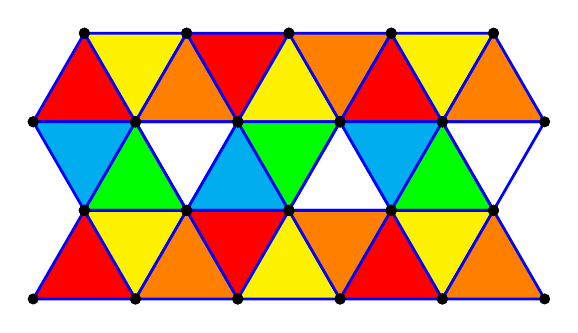
\begin{tikzpicture}[element/.style = {regular
polygon, regular polygon sides=3, draw=blue, line width=1pt, 
inner sep = 0, outer sep = 0, minimum size = 1.5cm},
dof/.style = {circle, inner sep=0, fill=black, minimum size = 4pt}]

\node (A) [element, fill=red] at
(0,0) {};
\node (B) [element, anchor=corner 1, rotate=180, fill=yellow] at
(A.corner 3) {};
\node (C) [element, anchor=corner 2,fill=orange] at (A.corner 3) {};
\node (D) [element, anchor=corner 1, rotate=180, fill=red] at
(C.corner 3) {};
\node (E) [element, anchor=corner 2, fill=yellow] at (C.corner 3) {};

\node (F) [element, anchor=corner 1, rotate=180, fill=orange] at
(E.corner 3) {};
\node (G) [element, anchor=corner 2, fill=red] at (E.corner 3) {};

\node (H) [element, anchor=corner 1, rotate=180, fill=yellow] at
(G.corner 3) {};
\node (I) [element, anchor=corner 2, fill=orange] at (G.corner 3) {};

\node (A1) [element, rotate=180, anchor=corner 3, fill=cyan] at
(A.corner 2) {};
\node (B1) [element, anchor=corner 2, fill=green] at
(A1.corner 1) {};

\node (C1) [element, rotate=180, anchor=corner 3] at
(C.corner 2) {};
\node (D1) [element, anchor=corner 2, fill=cyan] at
(C1.corner 1) {};

\node (E1) [element, rotate=180, anchor=corner 3, fill=green] at
(E.corner 2) {};
\node (F1) [element, anchor=corner 2] at
(E1.corner 1) {};

\node (G1) [element, rotate=180, anchor=corner 3, fill=cyan] at
(G.corner 2) {};
\node (H1) [element, anchor=corner 2, fill=green] at
(G1.corner 1) {};
\node (I1) [element, rotate=180, anchor=corner 3] at
(I.corner 2) {};

\node (A2) [element, anchor=corner 1, fill=red] at
(A1.corner 1) {};
\node (B2) [element, anchor=corner 1, rotate=180, fill=yellow] at
(A2.corner 3) {};
\node (C2) [element, anchor=corner 2, fill=orange] at (A2.corner 3) {};
\node (D2) [element, anchor=corner 1, rotate=180, fill=red] at
(C2.corner 3) {};
\node (E2) [element, anchor=corner 2, fill=yellow] at (C2.corner 3) {};

\node (F2) [element, anchor=corner 1, rotate=180, fill=orange] at
(E2.corner 3) {};
\node (G2) [element, anchor=corner 2, fill=red] at (E2.corner 3) {};

\node (H2) [element, anchor=corner 1, rotate=180, fill=yellow] at
(G2.corner 3) {};
\node (I2) [element, anchor=corner 2, fill=orange] at (G2.corner 3) {};

\foreach \ele in {A, B, C, D, E, F, G, H, I,
                  A1, B1, C1, D1, E1, F1, G1, H1,
                  A2, B2, C2, D2, E2, F2, G2, H2, I2}
\foreach \val in {corner 1, corner 2, corner 3}
\node [dof] at (\ele.\val) {};
\end{tikzpicture}
}

\only<7>{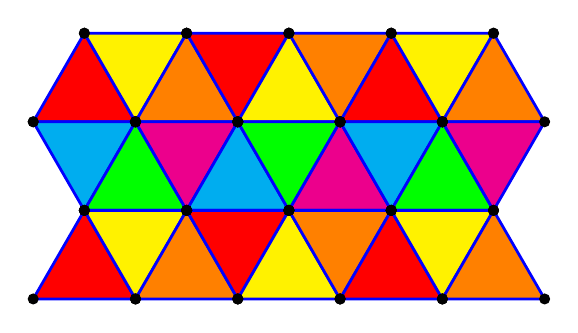
\begin{tikzpicture}[element/.style = {regular
polygon, regular polygon sides=3, draw=blue, line width=1pt, 
inner sep = 0, outer sep = 0, minimum size = 1.5cm},
dof/.style = {circle, inner sep=0, fill=black, minimum size = 4pt}]

\node (A) [element, fill=red] at
(0,0) {};
\node (B) [element, anchor=corner 1, rotate=180, fill=yellow] at
(A.corner 3) {};
\node (C) [element, anchor=corner 2,fill=orange] at (A.corner 3) {};
\node (D) [element, anchor=corner 1, rotate=180, fill=red] at
(C.corner 3) {};
\node (E) [element, anchor=corner 2, fill=yellow] at (C.corner 3) {};

\node (F) [element, anchor=corner 1, rotate=180, fill=orange] at
(E.corner 3) {};
\node (G) [element, anchor=corner 2, fill=red] at (E.corner 3) {};

\node (H) [element, anchor=corner 1, rotate=180, fill=yellow] at
(G.corner 3) {};
\node (I) [element, anchor=corner 2, fill=orange] at (G.corner 3) {};

\node (A1) [element, rotate=180, anchor=corner 3, fill=cyan] at
(A.corner 2) {};
\node (B1) [element, anchor=corner 2, fill=green] at
(A1.corner 1) {};

\node (C1) [element, rotate=180, anchor=corner 3, fill=magenta] at
(C.corner 2) {};
\node (D1) [element, anchor=corner 2, fill=cyan] at
(C1.corner 1) {};

\node (E1) [element, rotate=180, anchor=corner 3, fill=green] at
(E.corner 2) {};
\node (F1) [element, anchor=corner 2, fill=magenta] at
(E1.corner 1) {};

\node (G1) [element, rotate=180, anchor=corner 3, fill=cyan] at
(G.corner 2) {};
\node (H1) [element, anchor=corner 2, fill=green] at
(G1.corner 1) {};
\node (I1) [element, rotate=180, anchor=corner 3, fill=magenta] at
(I.corner 2) {};

\node (A2) [element, anchor=corner 1, fill=red] at
(A1.corner 1) {};
\node (B2) [element, anchor=corner 1, rotate=180, fill=yellow] at
(A2.corner 3) {};
\node (C2) [element, anchor=corner 2, fill=orange] at (A2.corner 3) {};
\node (D2) [element, anchor=corner 1, rotate=180, fill=red] at
(C2.corner 3) {};
\node (E2) [element, anchor=corner 2, fill=yellow] at (C2.corner 3) {};

\node (F2) [element, anchor=corner 1, rotate=180, fill=orange] at
(E2.corner 3) {};
\node (G2) [element, anchor=corner 2, fill=red] at (E2.corner 3) {};

\node (H2) [element, anchor=corner 1, rotate=180, fill=yellow] at
(G2.corner 3) {};
\node (I2) [element, anchor=corner 2, fill=orange] at (G2.corner 3) {};

\foreach \ele in {A, B, C, D, E, F, G, H, I,
                  A1, B1, C1, D1, E1, F1, G1, H1,
                  A2, B2, C2, D2, E2, F2, G2, H2, I2}
\foreach \val in {corner 1, corner 2, corner 3}
\node [dof] at (\ele.\val) {};
\end{tikzpicture}
}
\end{center}
\end{frame}

\begin{frame}[fragile,label={sec:orgheadline22}]{Does it work?}
 \begin{itemize}
\item Yes, elements with identical colours may safely be assembled in
parallel
\end{itemize}

\begin{minted}[frame=none,xleftmargin=1em,xrightmargin=1em,fontsize=\scriptsize]{fortran}
do c = 1, ncol
   nele = len(col(c))
   !$OMP PARALLEL do
   do i = 1, nele
      ele = fetch(col(c), i)
      localtensor = assemble(ele)
      ! race free
      call addto(local_tensor, big_matrix)
   end do
end do
\end{minted}
\end{frame}

\section{\ldots{}with halo data}
\label{sec:orgheadline28}
\begin{frame}[label={sec:orgheadline24}]{But what about halo data?}
\begin{itemize}
\item In an MPI parallel simulation, things are more complicated
\item Not all the dofs are local (some are in the halo)
\end{itemize}

\begin{center}


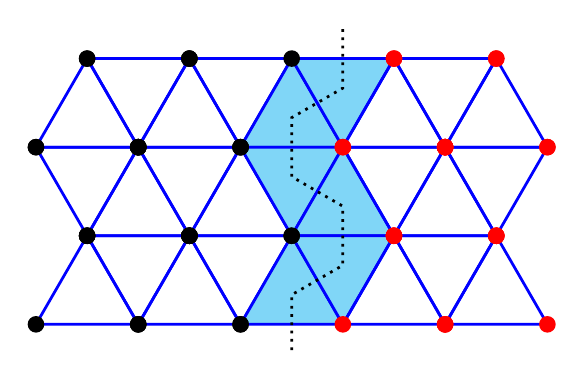
\begin{tikzpicture}[element/.style = {regular
polygon, regular polygon sides=3, draw=blue, line width=1pt, 
inner sep = 0, outer sep = 0, minimum size = 1.5cm},
dof1/.style={circle, fill=black, inner sep=0, minimum size = 6pt},
dof2/.style={circle, fill=red, inner sep=0, minimum size = 6pt},
halo/.style = {fill=cyan!50}]


\node (A) [element] at
(0,0) {};
\node (B) [element, anchor=corner 1, rotate=180] at
(A.corner 3) {};
\node (C) [element, anchor=corner 2] at (A.corner 3) {};
\node (D) [element, anchor=corner 1, rotate=180] at
(C.corner 3) {};
\node (E) [element, halo, anchor=corner 2] at (C.corner 3) {};

\node (F) [element, halo, anchor=corner 1, rotate=180] at
(E.corner 3) {};
\node (G) [element, anchor=corner 2] at (E.corner 3) {};

\node (H) [element, anchor=corner 1, rotate=180] at
(G.corner 3) {};
\node (I) [element, anchor=corner 2] at (G.corner 3) {};

\node (A1) [element, rotate=180, anchor=corner 3] at
(A.corner 2) {};
\node (B1) [element, anchor=corner 2] at
(A1.corner 1) {};

\node (C1) [element, rotate=180, anchor=corner 3] at
(C.corner 2) {};
\node (D1) [element, anchor=corner 2] at
(C1.corner 1) {};

\node (E1) [element, halo, rotate=180, anchor=corner 3] at
(E.corner 2) {};
\node (F1) [element, halo, anchor=corner 2] at
(E1.corner 1) {};

\node (G1) [element, rotate=180, anchor=corner 3] at
(G.corner 2) {};
\node (H1) [element, anchor=corner 2] at
(G1.corner 1) {};
\node (I1) [element, rotate=180, anchor=corner 3] at
(I.corner 2) {};

\node (A2) [element, anchor=corner 1] at
(A1.corner 1) {};
\node (B2) [element, anchor=corner 1, rotate=180] at
(A2.corner 3) {};
\node (C2) [element, anchor=corner 2] at (A2.corner 3) {};
\node (D2) [element, anchor=corner 1, rotate=180] at
(C2.corner 3) {};
\node (E2) [element, halo, anchor=corner 2] at (C2.corner 3) {};

\node (F2) [element, halo, anchor=corner 1, rotate=180] at
(E2.corner 3) {};
\node (G2) [element, anchor=corner 2] at (E2.corner 3) {};

\node (H2) [element, anchor=corner 1, rotate=180] at
(G2.corner 3) {};
\node (I2) [element, anchor=corner 2] at (G2.corner 3) {};

\foreach \ele in {A, B, C, D,
                  A1, B1, C1, D1,
                  A2, B2, C2, D2}
\foreach \val in {corner 1, corner 2, corner 3}
\node [dof1] at (\ele.\val) {};


\foreach \ele in {G, H, I, G1, H1, I1, G2, H2, I2}
\foreach \val in {corner 1, corner 2, corner 3}
\node [dof2] at (\ele.\val) {};

\draw [line width=1, dotted] (intersection cs:
first line={(E.corner 1)--($(E.corner 1) + (30:3)$)},
second line={(G.corner 1)--($(G.corner 1) + (150:3)$)}) -- (F.center)
-- (E.center) -- (E1.center) -- (F1.center) -- (F2.center) --
(E2.center) --(intersection cs:
first line = {(E2.corner 2) -- ($(E2.corner 2) +(-30:3)$)},
second line = {(E2.corner 3) -- ($(E2.corner 3)+(-150:3)$)});

\end{tikzpicture}
\end{center}

\begin{itemize}
\item What to do with contributions to non-local dofs?
\end{itemize}
\end{frame}

\begin{frame}[label={sec:orgheadline25}]{What Fluidity does}
\begin{itemize}
\item CG
\begin{itemize}
\item assemble \emph{all} elements (including those in halo)
\item contributions to non-local dofs are thrown away
\end{itemize}
\item DG
\begin{itemize}
\item assemble \emph{only} owned elements (don't assemble in halo)
\item contributions to non-local dofs are communicated
\end{itemize}
\item FV/CV
\begin{itemize}
\item I don't know, looks like CG (I think)
\end{itemize}
\end{itemize}
\end{frame}

\begin{frame}[fragile,label={sec:orgheadline26}]{How does the communication work?}
 \begin{itemize}
\item Local dofs get written directly into the matrix
\item Non-local dofs get written to a \emph{single} stash
\end{itemize}
\begin{minted}[frame=none,xleftmargin=1em,xrightmargin=1em,fontsize=\scriptsize,mathescape]{fortran}
subroutine addto(ltensor, m)
  ...
  if (islocal(i,j)) then
     m%data(i,j) = ltensor(i,j)
  else
     ! race condition
     m%stash(k)=stash_entry(ltensor(i,j), i,j)
     k = k+1
  end if
  ...
end subroutine addto
\end{minted}
\begin{itemize}
\item stash is communicated in one go at end of assembly loop
\end{itemize}
\end{frame}

\begin{frame}[label={sec:orgheadline27}]{More problems (+ solution)}
\begin{itemize}
\item Stashing code is in third-party library (PETSc)
\item Need a solution in Fluidity
\begin{itemize}
\item DG assembly now assembles in local + L1 element halo
\item this is enough for correctness (draw lots of pictures)
\end{itemize}
\end{itemize}
\end{frame}

\section{Was it worth it?}
\label{sec:orgheadline30}
\begin{frame}[fragile,label={sec:orgheadline29}]{Always good for strong scaling}
 \begin{itemize}
\item No longer need to do any communication when assembling matrix
\item Previously, one \texttt{MPI\_Allreduce} and one \texttt{MPI\_Alltoallv}
\item Assumption: we had the halo data anyway
\end{itemize}

\begin{center}
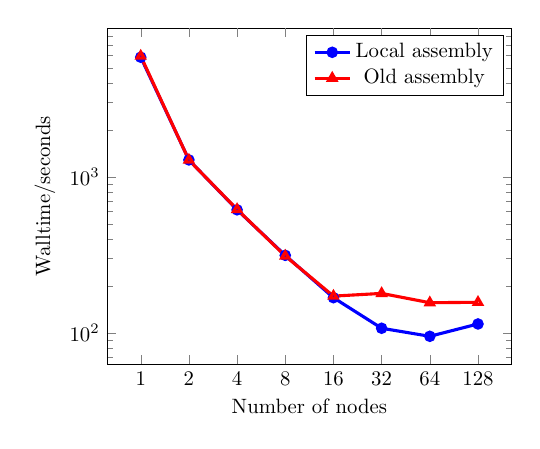
\begin{tikzpicture}[scale=0.75]
\begin{loglogaxis}[xlabel=Number of nodes,
ylabel=Walltime/seconds, xtick={1},
xticklabels={1},
extra x tick labels = {2, 4, 8, 16, 32, 64, 128},
extra x ticks = {2,4, 8, 16, 32, 64, 128}]

\addplot[color=blue,mark=*, line width=1.5pt] plot coordinates {
(1, 5854)
(2, 1285)
(4, 615)
(8, 314)
(16, 168)
(32, 107)
(64, 95)
(128, 114)
};

\addlegendentry{Local assembly}

\addplot[color=red, line width=1.5pt, mark=triangle] plot coordinates {
(1, 5952)
(2, 1282)
(4, 619)
(8, 311)
(16, 172)
(32, 179)
(64, 156)
(128, 157)
};
\addlegendentry{Old assembly}
\end{loglogaxis}
\end{tikzpicture}
\end{center}
\end{frame}
\section{What else can we do?}
\label{sec:orgheadline32}
\begin{frame}[label={sec:orgheadline31}]{Room for improvement}
\begin{itemize}
\item Element-wise colouring destroys any cache locality
\item Assuming there was any
\begin{itemize}
\item work ongoing to improve mesh entity numbering
\end{itemize}
\item To exploit this:
\begin{itemize}
\item construct mini-partitions on each node
\item colour partitions
\end{itemize}
\item Each thread gets a mini-partition of the same colour
\begin{itemize}
\item more cache friendly
\end{itemize}
\end{itemize}
\end{frame}

\section{Some guidelines/advice}
\label{sec:orgheadline39}
\begin{frame}[fragile,label={sec:orgheadline33}]{Other things to think about}
 \begin{itemize}
\item Many things in Fluidity are not thread-safe
\item Reference counting
\begin{itemize}
\item Any time you do \texttt{call allocate(...)}
\end{itemize}
\item Populating data caches
\begin{itemize}
\item \texttt{transform\_to\_physical} has a cache
\end{itemize}
\item Anything that updates module-level variables
\begin{itemize}
\item e.g. \texttt{set\_coriolis\_parameters}
\end{itemize}
\item Other functionality may be, but I don't know
\end{itemize}
\end{frame}

\begin{frame}[fragile,label={sec:orgheadline34}]{Things to think about II}
 \begin{itemize}
\item Fortunately, these shouldn't occur in potential threaded code anyway
\item \texttt{allocate} in assembly loop is \emph{bad}
\item For lazy cache population, force it in unthreaded code
\end{itemize}

\begin{minted}[frame=none,xleftmargin=1em,xrightmargin=1em,fontsize=\scriptsize]{fortran}
call prepopulate_transform_cache(field)
...
!$OMP parallel
! no race condition reading from the cache
call transform_to_physical(...)
!$OMP end parallel
\end{minted}
\end{frame}

\begin{frame}[fragile,label={sec:orgheadline35}]{How do I know I'm doing it wrong}
 \begin{itemize}
\item For known thread-unsafe code, Fluidity will abort
\end{itemize}
\begin{minted}[frame=none,xleftmargin=1em,xrightmargin=1em,fontsize=\scriptsize]{fortran}
subroutine unsafe()
  ! in Parallel_Tools
  call abort_if_in_parallel_region
  ...
end subroutine unsafe
subroutine foo()
  ...
  !$OMP parallel
  call unsafe()                 ! aborts
end subroutine foo
\end{minted}
\begin{itemize}
\item If you add new functionality that is not safe, mark it
\end{itemize}
\end{frame}

\begin{frame}[fragile,label={sec:orgheadline36}]{Finding/fixing threading bugs}
 \begin{itemize}
\item tests may fail if run with \texttt{OMP\_NUM\_THREADS > 1}
\begin{itemize}
\item but not always!
\end{itemize}
\item valgrind has two tools
\begin{itemize}
\item \texttt{valgrind -{}-tool=drd}
\item \texttt{valgrind -{}-tool=helgrind}
\end{itemize}
\item think hard!
\begin{itemize}
\item even harder than for MPI
\item less preferable, but more accurate than valgrind
\end{itemize}
\end{itemize}
\end{frame}

\begin{frame}[label={sec:orgheadline37}]{Summary}
\begin{itemize}
\item Fluidity updated to support (lock-free) hybrid matrix assembly
\begin{itemize}
\item AD CG, Momentum CG/DG (threaded)
\item in trunk as of r3984
\end{itemize}
\item Assembly routines "localised" (no comms)
\item Ongoing work to hybridise linear solver (PETSc)
\begin{itemize}
\item \href{http://arxiv.org/abs/1205.2005}{arXiv:1205.2005 [cs.DC]}
\end{itemize}
\item Performance looks good
\begin{itemize}
\item work on cache optimisation should improve things
\end{itemize}
\item Shared memory programming is hard
\begin{itemize}
\item can/should we use higher-level approaches?
\end{itemize}
\end{itemize}
\end{frame}

\begin{frame}[label={sec:orgheadline38}]{Acknowledgments}
\begin{itemize}
\item Michele Weiland (EPCC)
\item Gerard Gorman, David Ham, Stefan Kramer (AMCG)
\item Xiaohu Guo (STFC Daresbury)
\item Any others I may have forgotton (various)
\end{itemize}
\end{frame}
\end{document}
